\documentclass{article}
\usepackage{amsmath,amssymb}
\usepackage{tikz}
\usetikzlibrary{calc}
\setlength{\parindent}{0pt}

\begin{document}

\textbf{MATH 1564 --- Notes 09/17}

\bigskip

\textbf{Theorem.} The usual algorithm for solving $Ax=0$ and writing the solution in parametric vector form gives a basis for $\operatorname{Nul} A$.

\medskip

\textbf{Theorem.} The pivot columns of $A$ form a basis for $\operatorname{Col} A$.

\medskip

\textbf{Example.} Let $A=[a_1\ a_2\ a_3\ a_4]$, where
\[
A=
\begin{bmatrix}
1&1&-1&1\\
2&3&-1&0\\
2&3&-1&0
\end{bmatrix}
\sim
\begin{bmatrix}
1&1&-1&1\\
0&1&1&-2\\
0&0&0&0
\end{bmatrix}
\sim
R=
\begin{bmatrix}
1&0&-2&3\\
0&1&1&-2\\
0&0&0&0
\end{bmatrix}.
\]
The pivot columns are columns $1$ and $2$, so $\{a_1,a_2\}$ is a basis for $\operatorname{Col} A$.

\medskip

For $Rx=0$, the free variables are $x_3$ and $x_4$:
\[
r_3=-2r_1+r_2,\qquad r_4=3r_1-2r_2.
\]
Thus the dependence relations among the columns of $A$ are
\[
2a_1-a_2+a_3=0,
\qquad
-3a_1+2a_2+a_4=0.
\]
Equivalently,
\[
\operatorname{Nul} A=\operatorname{span}\left\{
\begin{bmatrix}2\\-1\\1\\0\end{bmatrix},
\begin{bmatrix}-3\\2\\0\\1\end{bmatrix}
\right\}.
\]
In particular, $a_3$ and $a_4$ are in $\operatorname{span}\{a_1,a_2\}$.

\newpage

\textbf{Examples of bases}

\medskip

\textbf{Example.} What is a basis for $\{0\}$, the zero subspace of $\mathbb{R}^n$?

\medskip

The empty set is a basis: it spans $\{0\}$, and it has no dependent vectors. The set $\{0\}$ itself is not a basis because the zero vector is always dependent.

\medskip

\textbf{Example.} If $S$ is a nonzero subspace of $\mathbb{R}^n$, how many bases does $S$ have?

\medskip

Infinitely many. If $\{v_1,\ldots,v_k\}$ is a basis, then so are, for example,
\[
\{2v_1,\ldots,2v_k\},\quad \{3v_1,\ldots,3v_k\},\quad \ldots
\]

\medskip

\textbf{Basis as a grid.} A basis gives coordinate directions. In the standard basis of $\mathbb{R}^2$, $e_1$ and $e_2$ determine a rectangular grid; for example, $e_2+3e_1$ is located by moving $3$ units in the $e_1$ direction and $1$ unit in the $e_2$ direction. A nonstandard basis $\{v_1,v_2\}$ produces a skew grid, but it still gives unique coordinates.

\begin{center}
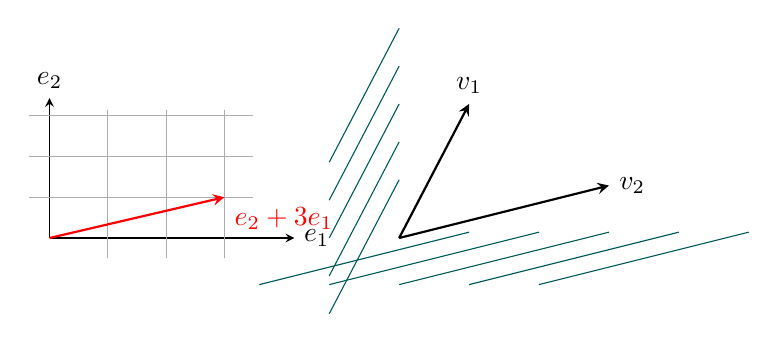
\begin{tikzpicture}[scale=.74,>=stealth]
\draw[->] (0,0)--(4.2,0) node[right] {$e_1$};
\draw[->] (0,0)--(0,2.4) node[above] {$e_2$};
\foreach \x in {1,2,3} \draw[gray!65] (\x,-.35)--(\x,2.2);
\foreach \y in {.7,1.4,2.1} \draw[gray!65] (-.35,\y)--(3.5,\y);
\draw[red,->,thick] (0,0)--(3,.7) node[below right] {$e_2+3e_1$};
\begin{scope}[xshift=6cm]
\draw[->,thick] (0,0)--(3.6,.9) node[right] {$v_2$};
\draw[->,thick] (0,0)--(1.2,2.3) node[above] {$v_1$};
\foreach \t in {-2,-1,0,1,2} \draw[teal!70!black] (\t*1.2,-.8)--($(\t*1.2,-.8)+(3.6,.9)$);
\foreach \t in {-2,-1,0,1,2} \draw[teal!70!black] (-1.2,\t*.65)--($(-1.2,\t*.65)+(1.2,2.3)$);
\end{scope}
\end{tikzpicture}
\end{center}

\newpage

\textbf{Coordinates relative to a basis}

\medskip

\textbf{Definition.} Let $\beta=\{b_1,\ldots,b_k\}$ be a basis for a subspace $S$. For $x\in S$, its coordinates relative to $\beta$ are the scalars $c_1,\ldots,c_k$ such that
\[
x=c_1b_1+\cdots+c_kb_k.
\]
We write
\[
[x]_\beta=
\begin{bmatrix}c_1\\ \vdots\\ c_k\end{bmatrix}.
\]

\medskip

\textbf{Example.} Let
\[
v_1=\begin{bmatrix}1\\1\end{bmatrix},
\qquad
v_2=\begin{bmatrix}1\\-1\end{bmatrix}.
\]
Then $\{v_1,v_2\}$ is a basis of $\mathbb{R}^2$: indeed,
\[
e_1=\frac{v_1+v_2}{2},
\qquad
e_2=\frac{v_1-v_2}{2}.
\]
Thus the vectors span $\mathbb{R}^2$, and their independence is clear.

\medskip

Find the coordinates of $e_1=\begin{bmatrix}1\\0\end{bmatrix}$ in $\beta=\{v_1,v_2\}$. If
\[
[e_1]_\beta=\begin{bmatrix}c_1\\c_2\end{bmatrix},
\]
then
\[
\begin{bmatrix}1\\0\end{bmatrix}
=
\begin{bmatrix}1&1\\1&-1\end{bmatrix}
\begin{bmatrix}c_1\\c_2\end{bmatrix}.
\]
Therefore,
\[
\begin{bmatrix}c_1\\c_2\end{bmatrix}
=
\begin{bmatrix}1&1\\1&-1\end{bmatrix}^{-1}
\begin{bmatrix}1\\0\end{bmatrix}
=\frac{1}{-2}
\begin{bmatrix}-1&-1\\-1&1\end{bmatrix}
\begin{bmatrix}1\\0\end{bmatrix}
=\begin{bmatrix}\tfrac12\\\tfrac12\end{bmatrix}.
\]

\newpage

\textbf{Theorem.} $x$ and $\beta$ determine $[x]_\beta$.

\medskip

\textbf{Proof.} Suppose $\beta=\{b_1,\ldots,b_k\}$ and
\[
x=c_1b_1+\cdots+c_kb_k=d_1b_1+\cdots+d_kb_k.
\]
Then
\[
\begin{bmatrix}c_1\\ \vdots\\ c_k\end{bmatrix}
=
\begin{bmatrix}d_1\\ \vdots\\ d_k\end{bmatrix},
\]
because $\beta$ is linearly independent. Hence the coordinate vector is unique.

\bigskip

\textbf{Dimension}

\medskip

\textbf{Definition.} The dimension of a subspace $S\subseteq\mathbb{R}^n$ is the number of vectors in a basis of $S$.

\medskip

\textbf{Examples.}
\begin{itemize}
\item $\dim(\mathbb{R}^n)=n$, since $\{e_1,\ldots,e_n\}$ is a basis.
\item $\dim\{0\}=0$.
\item $\dim(\operatorname{Col} A)$ is the number of pivots of $A$.
\item $\dim(\operatorname{Nul} A)$ is the number of free variables, equivalently the number of nonpivot columns.
\end{itemize}

\medskip

For
\[
S=\left\{\begin{bmatrix}x_1\\ \vdots\\x_n\end{bmatrix}\in\mathbb{R}^n:x_1+\cdots+x_n=0\right\},
\]
we have $S=\operatorname{Nul} A$, where $A=\begin{bmatrix}1&\cdots&1\end{bmatrix}$. Since there is one pivot and $n-1$ free variables,
\[
\dim S=n-1.
\]

\newpage

\textbf{Theorem.} Let $S$ be a subspace of $\mathbb{R}^n$. Any two bases of $S$ have the same number of vectors.

\medskip

\textbf{Proof.} Let $\{a_1,\ldots,a_k\}$ and $\{b_1,\ldots,b_\ell\}$ be bases of $S$. Assume, for a contradiction, that $k>\ell$. Since the $b_i$ span $S$, write
\[
a_i=c_{i1}b_1+\cdots+c_{i\ell}b_\ell=Bc_i,
\]
where
\[
B=[b_1\ \cdots\ b_\ell],
\qquad
C=[c_1\ \cdots\ c_k].
\]
Then
\[
A=[a_1\ \cdots\ a_k]=BC.
\]
The columns of $A$ are independent because they form a basis, so the columns of $C$ must be independent. Thus $C$, which has only $\ell$ rows, would need $k$ pivot columns. This is impossible when $\ell<k$. Therefore $k\leq\ell$; reversing the roles of the two bases gives $\ell\leq k$, so $k=\ell$.

\bigskip

\textbf{Example.} If $A$ is a $5\times 7$ matrix, then
\[
\dim(\operatorname{Col} A)\leq 5,
\qquad
\dim(\operatorname{Nul} A)\geq 2.
\]

\medskip

\textbf{Definition.} The rank of $A$ is the number of pivots of $A$.

\medskip

If $T(x)=Ax$, then the image of $T$ is $\operatorname{Col} A$, which is a subspace, and
\[
\dim(\operatorname{image} T)=\operatorname{rank}(A).
\]

\newpage

\textbf{Rank Theorem.} If $T:\mathbb{R}^n\to\mathbb{R}^m$ is a linear map, then
\[
\dim(\operatorname{image} T)+\dim(\ker T)=n.
\]

\textbf{Proof.} Let $T(x)=Ax$. Then
\[
\operatorname{image} T=\operatorname{Col} A,
\qquad
\ker T=\operatorname{Nul} A.
\]
The dimension of $\operatorname{Col} A$ is the number of pivot columns, and the dimension of $\operatorname{Nul} A$ is the number of nonpivot columns. Every column is one or the other, so their dimensions add to $n$.

\medskip

\textbf{Example.} Let
\[
T(x_1,x_2,x_3)=2x_1-x_2+x_3.
\]
This is linear because $T(x)=Ax$, where
\[
A=\begin{bmatrix}2&-1&1\end{bmatrix}.
\]
Then
\[
\dim(\operatorname{image} T)=\dim(\operatorname{Col} A)=1,
\qquad
\dim(\ker T)=\dim(\operatorname{Nul} A)=2.
\]

\bigskip

Recall: a basis of a subspace $S$ is a set of independent vectors that spans $S$.

\medskip

\textbf{Theorem.} Let $v_1,\ldots,v_k\in S$, where $\dim S=k$. The following are equivalent:
\begin{enumerate}
\item $\{v_1,\ldots,v_k\}$ is a basis of $S$.
\item $S=\operatorname{span}\{v_1,\ldots,v_k\}$.
\item $\{v_1,\ldots,v_k\}$ is linearly independent.
\end{enumerate}

\medskip

By definition, (1) implies both (2) and (3), and (2) together with (3) implies (1).

\medskip

For (2) $\Rightarrow$ (3), the pivot columns of $[v_1\ \cdots\ v_k]$ form a basis of $\operatorname{Col}[v_1\ \cdots\ v_k]=S$. Since $\dim S=k$, there are $k$ pivots, so every column is pivotal.

\medskip

For (3) $\Rightarrow$ (2), if $\operatorname{span}\{v_1,\ldots,v_k\}\neq S$, choose $v_{k+1}\in S$ outside that span. Then $\{v_1,\ldots,v_k,v_{k+1}\}$ is independent. Repeating would create an independent set in $\mathbb{R}^n$ with more than $n$ vectors, which is impossible.

\newpage

Let $S_i=\operatorname{span}\{v_1,\ldots,v_i\}$, with $\{v_1,\ldots,v_i\}$ independent. Then
\[
S_k\subsetneq S_{k+1}\subsetneq S_{k+2}\subsetneq\cdots\subseteq S\subseteq\mathbb{R}^n.
\]

\textbf{Lemma.} $\mathbb{R}^n$ contains at most $n$ linearly independent vectors.

\medskip

\textbf{Proof.} If $\{v_1,\ldots,v_k\}\subseteq\mathbb{R}^n$ is independent, then the $n\times k$ matrix $[v_1\ \cdots\ v_k]$ has $k$ pivots. Hence $k\leq n$.

\medskip

Eventually, the process above must stop. At that point $S_i=S$, so $\{v_1,\ldots,v_i\}$ is a basis of $S$. This proves the equivalence theorem.

\bigskip

\textbf{Theorem.} Every nonzero subspace of $\mathbb{R}^n$ has a basis.

\medskip

\textbf{Proof.} Pick any nonzero $v_1\in S$ and let $S_1=\operatorname{span}\{v_1\}$. If $S=S_1$, then $\{v_1\}$ is a basis. Otherwise, choose $v_2\in S\setminus S_1$; then $\{v_1,v_2\}$ is independent. Continue: if
\[
S_i=\operatorname{span}\{v_1,\ldots,v_i\}\neq S,
\]
choose $v_{i+1}\in S\setminus S_i$. The lemma guarantees that this cannot continue past $n$ independent vectors. Therefore it stops with $S_i=S$, giving a basis.

\end{document}
